\begin{activity} \label{A:12.1.1}  
\nin The plot in Figure~\ref{fig:12.1.circle} illustrates the vector
field $\vF(x,y) = y\vi -x\vj$.
\begin{figure}[h]
  \centering
  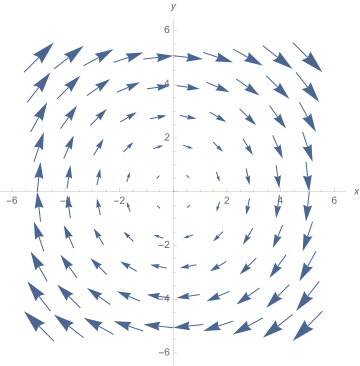
\includegraphics[width=0.35\linewidth]{12_1_circle.pdf}
  \caption{The vector field $y\vi-x\vj$}
  \label{fig:12.1.circle}
\end{figure}
\ba
\item Starting with one of the vectors near the point $(2,0)$, sketch
  a curve that follows the direction of the vector field $\vF$. To
  help visualize what you are doing, it may be useful to think of the
  vector field as the velocity vector field for some flowing water and
  that you are imagining tracing the path that a tiny particle
  inserted into the water would follow as the water moved it around.
\item Repeat the previous step for at least two other starting points
  not on the curve you previously sketched.
\item What shape do the curves you sketched in the previous two steps
  form?
\item Verify that $\vF(x,y)$ is orthogonal to $\langle x,y\rangle$.
\item What is the relationship between the function $f(x,y) = x^2 +
  y^2$ and the vector $x\vi + y\vj$? %(You might find it useful to
%  think about the vector $2x\vi + 2y\vj$ first.) 
\item What does this tell you about the relationship between
  $\vF(x,y)$ and circles centered at the origin?  What is the
  relationship between $|\vF(x,y)|$ and the radius of the appropriate circle?
\ea
\end{activity}
\begin{smallhint}

\end{smallhint}
\begin{bighint}

\end{bighint}
\begin{activitySolution}

\end{activitySolution}
\aftera
%%% Local Variables:
%%% mode: latex
%%% TeX-master: "../0_AC_MV"
%%% End:
